\begin{figure}[H]
    \centering

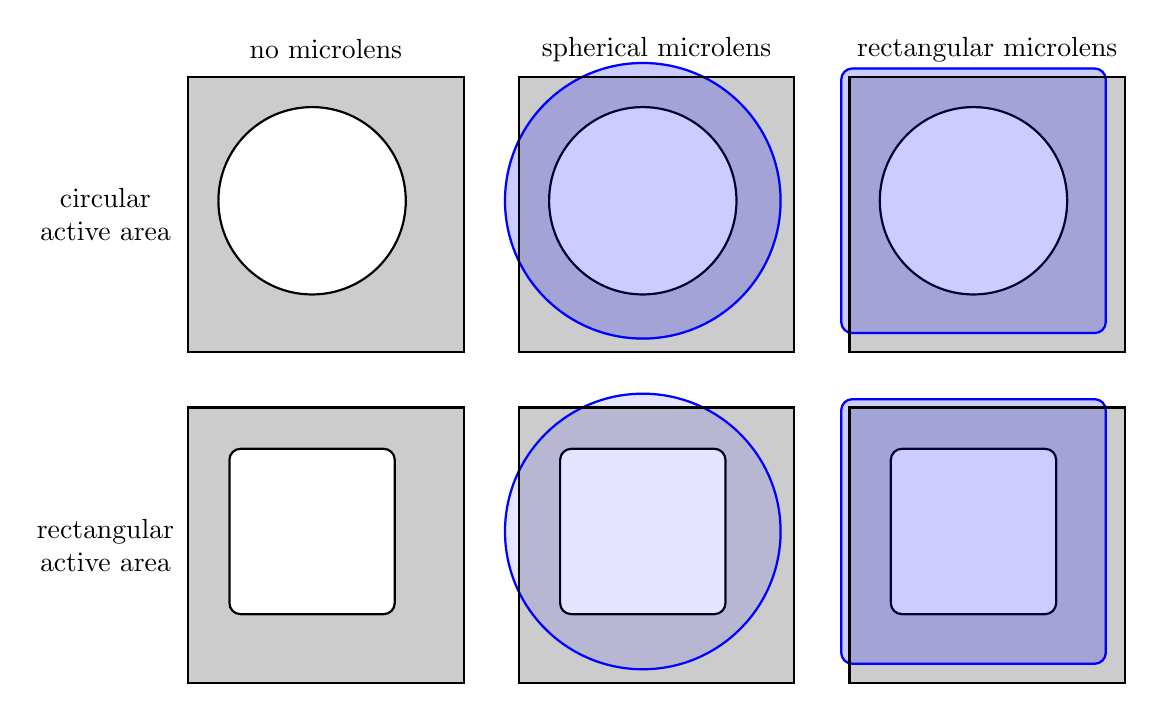
\begin{tikzpicture}[thick,scale=0.7, every node/.style={scale=1}]

\draw[fill, color=black!20]  (-1.25,3.25) rectangle (3.75,-1.75);
\draw[fill, color=white]  (1,1) ellipse (1.7 and 1.7);
\draw[]  (1,1) ellipse (1.7 and 1.7);

\draw[fill, color=black!20]  (4.75,3.25) rectangle (9.75,-1.75);
\draw[fill, color=white]  (7,1) ellipse (1.7 and 1.7);
\draw[]  (7,1) ellipse (1.7 and 1.7);
\draw [fill, color=blue, opacity=0.2] (7,1) ellipse (2.5 and 2.5);
\draw [color=blue] (7,1) ellipse (2.5 and 2.5);

\draw[fill, color=black!20]  (10.75,3.25) rectangle (15.75,-1.75);
\draw[fill, color=white]  (13,1) ellipse (1.7 and 1.7);
\draw[]  (13,1) ellipse (1.7 and 1.7);
\draw [fill, color=blue, opacity=0.2, rounded corners] (10.6,3.4) rectangle (15.4,-1.4);
\draw [color=blue, rounded corners] (10.6,3.4) rectangle (15.4,-1.4);

\draw[fill, color=black!20]  (-1.25,-2.75) rectangle (3.75,-7.75);
\draw[fill, color=white, rounded corners] (-0.5,-3.5) rectangle (2.5,-6.5) {};
\draw[rounded corners] (-0.5,-3.5) rectangle (2.5,-6.5) {};

\draw[fill, color=black!20]  (4.75,-2.75) rectangle (9.75,-7.75);
\draw[fill, color=white, rounded corners] (5.5,-3.5) rectangle (8.5,-6.5) {};
\draw[rounded corners] (5.5,-3.5) rectangle (8.5,-6.5) {};
\draw [fill, color=blue, opacity=0.1] (7,-5) ellipse (2.5 and 2.5);
\draw [color=blue] (7,-5) ellipse (2.5 and 2.5);

\draw[fill, color=black!20]  (10.75,-2.75) rectangle (15.75,-7.75);
\draw[fill, color=white, rounded corners] (11.5,-3.5) rectangle (14.5,-6.5) {};
\draw[rounded corners] (11.5,-3.5) rectangle (14.5,-6.5) {};
\draw [fill, color=blue, opacity=0.2, rounded corners] (10.6,-2.6) rectangle (15.4,-7.4);
\draw [color=blue, rounded corners] (10.6,-2.6) rectangle (15.4,-7.4);

\draw[]  (-1.25,3.25) rectangle (3.75,-1.75);
\draw[]  (4.75,3.25) rectangle (9.75,-1.75);
\draw[]  (10.75,3.25) rectangle (15.75,-1.75);

\draw[]  (-1.25,-2.75) rectangle (3.75,-7.75);
\draw[]  (4.75,-2.75) rectangle (9.75,-7.75);
\draw[]  (10.75,-2.75) rectangle (15.75,-7.75);

\node at (1.25,3.75) {no microlens};
\node at (7.25,3.75) {spherical microlens};
\node at (13.25,3.75) {rectangular microlens};
\node[align=center] at (-2.75,0.75) {circular\\active area};
\node[align=center] at (-2.75,-5.25) {rectangular\\active area};
\end{tikzpicture}
    \caption{Options for lenses with varying types of active areas and microlenses}
    \label{tkz:SPAD_types}
\end{figure}
